% 第 11 章 Using the Message Browser
\bichapter{使用消息浏览器}{Using the Message Browser}
\label{chap:gui-msg}

IC Compiler II GUI 提供增强消息系统（enhanced message system，EMS）数据库以及消息浏览器（message browser）工具，用来管理和查看与版图中规则违例（rule violation）有关的错误消息和信息性消息（informational message）。EMS 数据库由 \cmd{check\_design} 命令以及其他检查命令生成。使用消息浏览器时，可以选中单条消息，也可以按消息类型选择消息，在版图视图（layout view）中高亮受影响的对象，并为违例创建豁免（waiver）。消息浏览器还会为当前选中的消息显示 HTML 格式的手册页（man page）。如果有多个 EMS 数据库，消息浏览器可以把这些数据库合并成一个统一的数据库。

本章包括以下主题：
\begin{itemize}
  \item 准备 EMS 数据库
  \item 消息浏览器布局
  \item 重新分类消息
  \item 创建豁免
  \item 合并 EMS 数据库
\end{itemize}

\section{准备 EMS 数据库}
\subsection*{Preparing the EMS Database}

使用消息浏览器之前，必须先创建 EMS 数据库。

该数据库由设计检查工具生成，例如 \cmd{check\_design}、\cmd{check\_hier\_design}、\cmd{check\_netlist}、\cmd{check\_routability} 和 \cmd{check\_timing}。在检查命令之前运行 \cmd{create\_ems\_database} 命令，在检查命令之后运行 \cmd{save\_ems\_database} 命令。例如：
\begin{lstlisting}
icc2_shell> create_ems_database check_hier.ems
icc2_shell> check_hier_design -stage timing
icc2_shell> save_ems_database
\end{lstlisting}

在版图窗口中选择 \textbf{Window > Message Browser Window}，打开消息浏览器。也可以在 \cmd{check\_design} 命令上加上 \opt{-open\_message\_browser} 选项，使分析结束后自动打开消息浏览器。

\section{消息浏览器布局}
\subsection*{Message Browser Layout}

图~\ref{fig:gui-135} 标出了消息浏览器中的各个区域。

\begin{figure}[htbp]
\centering
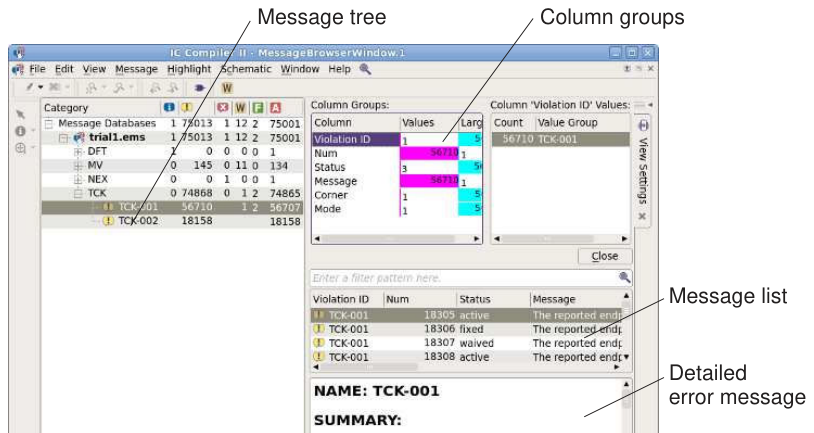
\includegraphics[width=0.92\textwidth]{gui-fig-135.png}
\caption{消息浏览器}
\label{fig:gui-135}
\end{figure}

以下几节说明消息浏览器中的各个窗格。

\subsection{消息树}
\subsubsection*{Message Tree}

消息树在浏览器左侧以树视图（tree view）列出错误，见图~\ref{fig:gui-136}。树视图显示当前 EMS 数据库的名称，以及数据库中错误与警告的层次。

\begin{figure}[htbp]
\centering
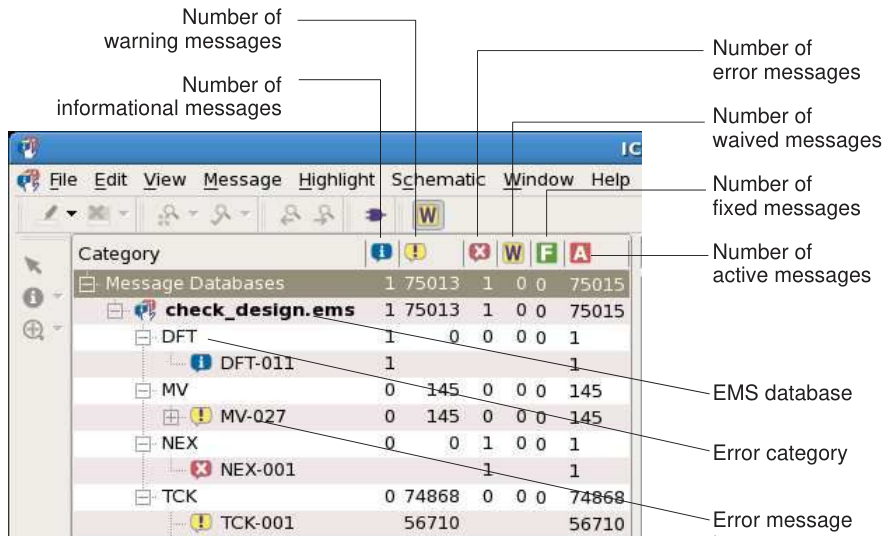
\includegraphics[width=0.92\textwidth]{gui-fig-136.png}
\caption{消息浏览器树}
\label{fig:gui-136}
\end{figure}

\subsection{消息列表}
\subsubsection*{Message List}

消息列表显示当前所选错误消息类型的完整消息列表，见图~\ref{fig:gui-137}。每个条目包括违例标识（Violation ID）、内部错误消息索引、当前状态（活动 active、已豁免 waived 或已修复 fixed）、消息文本，以及在有附加信息时一并给出的内容。把鼠标指针移到某一消息行上，可以查看该消息的更多信息。单击列表中的一行即可选中它。选中消息行之后，工具会更新详细错误消息的显示。单击并拖动指针可以选中多行；也可以在单击某一行时按住 Shift 或 Control 键，把该行加入选择。按 Control-A 选中全部行。

\begin{figure}[htbp]
\centering
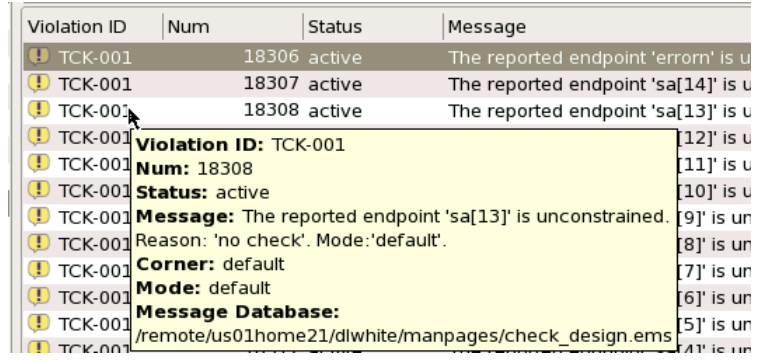
\includegraphics[width=0.92\textwidth]{gui-fig-137.png}
\caption{消息列表}
\label{fig:gui-137}
\end{figure}

在消息区域单击鼠标右键，显示上下文菜单（context menu）；从菜单中选择一项，可以执行下列操作：
\begin{itemize}
  \item Waive：把所选消息重新分类为已豁免；此操作只在当前会话中保留。
  \item Mark Fixed：把所选消息重新分类为已修复；此操作只在当前会话中保留。
  \item Mark Active：把所选消息重新分类为活动；此操作只在当前会话中保留。
  \item Select：在版图视图中选中相关对象。
  \item Highlight：在版图视图中高亮相关对象。
  \item Properties：显示该对象的属性。
  \item Show Column Groups：打开 Column Groups 窗格和 Column Status Values 窗格。
  \item Create Waiver：打开 Create Waiver 对话框；用该对话框创建豁免，见后文「创建豁免」。
  \item List Waivers：打开 Message Waivers 对话框；用该对话框显示当前的豁免列表。
  \item Copy：复制当前所选行的文本。
\end{itemize}

可以输入过滤模式，或使用列分组（column group）来过滤消息列表。在搜索框中输入字符时，工具会更新显示，只列出包含该搜索字符串的消息。

列分组把消息列表区域各列的信息计数组合成直方图（histogram）视图。数值列显示每一列有多少个互不相同的结果。在 Column Groups 框中单击某一行，右侧的列值区域会显示更多信息。在列值区域中单击某一行时，消息列表被过滤，只显示与当前所选值分组相匹配的消息。单击 Close 按钮，关闭列分组面板。列分组见图~\ref{fig:gui-138}。

\begin{figure}[htbp]
\centering
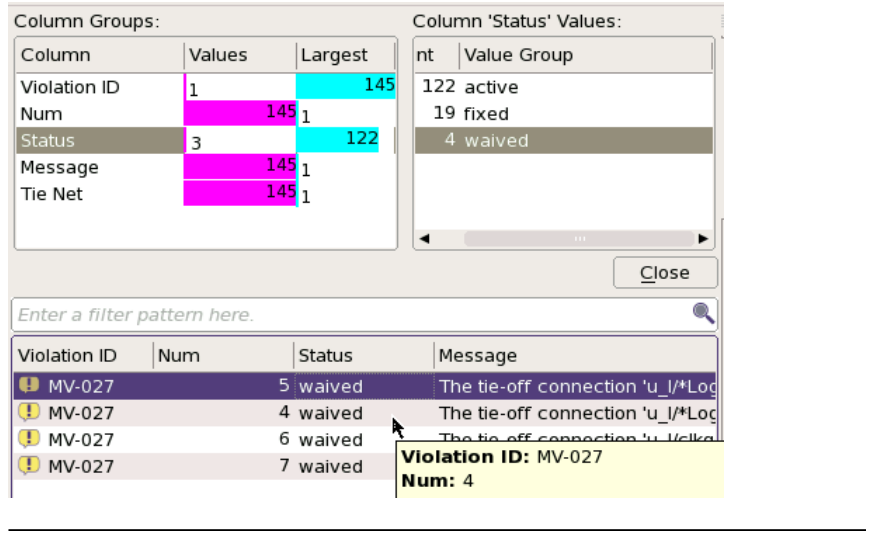
\includegraphics[width=0.92\textwidth]{gui-fig-138.png}
\caption{列分组}
\label{fig:gui-138}
\end{figure}

\subsection{详细错误消息}
\subsubsection*{Detailed Error Message}

消息浏览器显示当前所选错误的详细消息摘要和说明。在消息列表中单击不同的错误消息时，详细错误消息会显示该错误的消息摘要和详细说明。

要改变详细错误消息的位置，从菜单选择 \textbf{View > Html Pane}，然后选择 On Right 或 On Bottom。

\section{重新分类消息}
\subsection*{Reclassifying a Message}

使用消息浏览器，可以把单条消息重新分类为活动、已修复或已豁免。若只在当前会话中重新分类一条消息：
\begin{enumerate}
  \item 在树视图（Tree View）中选择该消息。
  \item 从 Message 菜单选择 Waive、Mark Fixed 或 Mark Active，见图~\ref{fig:gui-139}。也可以单击该消息，再从上下文菜单中选择相应操作。
\end{enumerate}
工具会更新列表视图中的计数。

\begin{figure}[htbp]
\centering
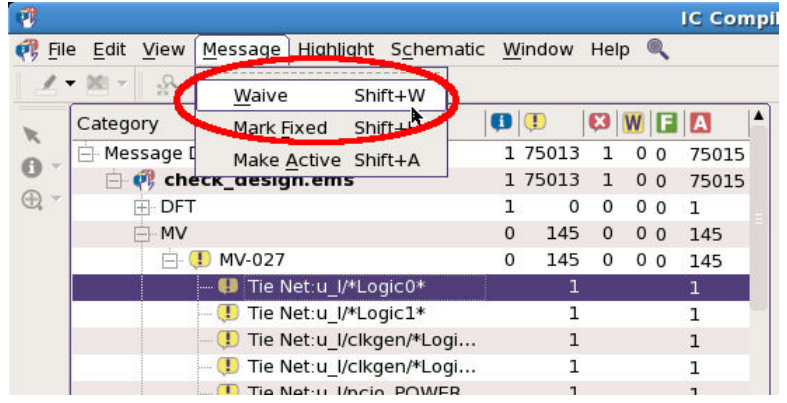
\includegraphics[width=0.92\textwidth]{gui-fig-139.png}
\caption{重新分类消息}
\label{fig:gui-139}
\end{figure}

\begin{noteBox}
这些更改只在当前会话中有效，退出消息浏览器时不会保存。
\end{noteBox}

\section{创建豁免}
\subsection*{Creating a Waiver}

为一条消息创建豁免，可以把附加信息关联到该消息上。这些信息不会保存到 EMS 数据库中。不过，可以把豁免写成 Tcl 命令，并在以后的会话中应用。要创建豁免：
\begin{enumerate}
  \item 选择要豁免的消息行。
  \item 右键单击，并从上下文菜单中选择 Create Waiver。\\
        工具在消息列表上方显示错误豁免表单（error waiver form），见图~\ref{fig:gui-140}。
  \item 在 Name 以及其他框中填写信息，完成错误豁免表单。标签前带星号（*）的框为必填项。
  \item 按需要修改条件（criteria）。\\
        单击加号按钮（+）添加条件，单击减号按钮（-）删除一条条件，或单击 Remove All 删除全部条件。
        \begin{noteBox}
        这些条件会应用于列表中的全部消息。
        \end{noteBox}
  \item 单击 Apply 创建豁免。\\
        工具把这些条件应用于列表中的全部消息，并把匹配消息的状态更新为 Waived。
\end{enumerate}

\begin{figure}[htbp]
\centering
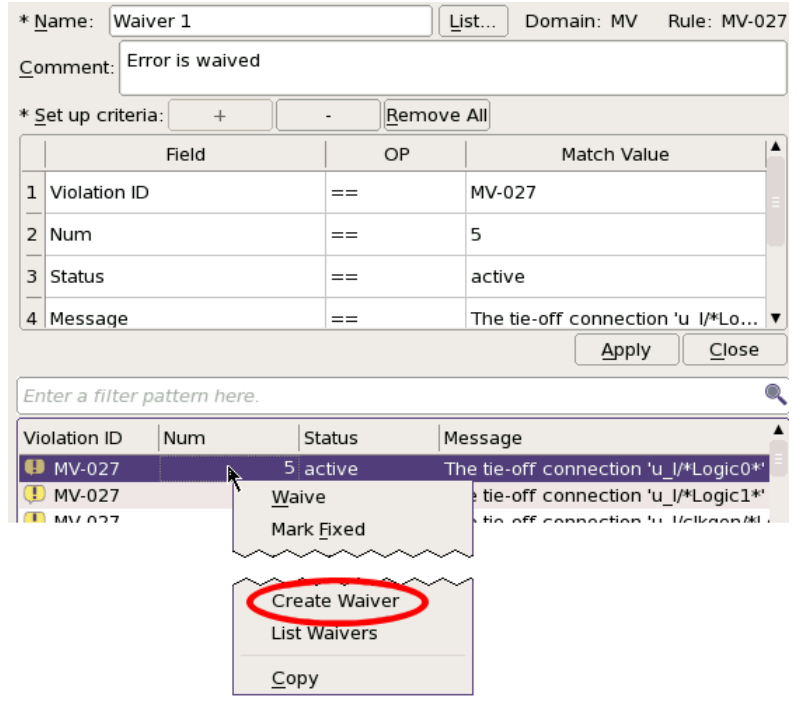
\includegraphics[width=0.92\textwidth]{gui-fig-140.png}
\caption{创建豁免}
\label{fig:gui-140}
\end{figure}

要显示当前会话的豁免列表，从菜单选择 \textbf{View > List Message Waivers}。工具会列出当前的豁免，见图~\ref{fig:gui-141}。

\begin{figure}[htbp]
\centering
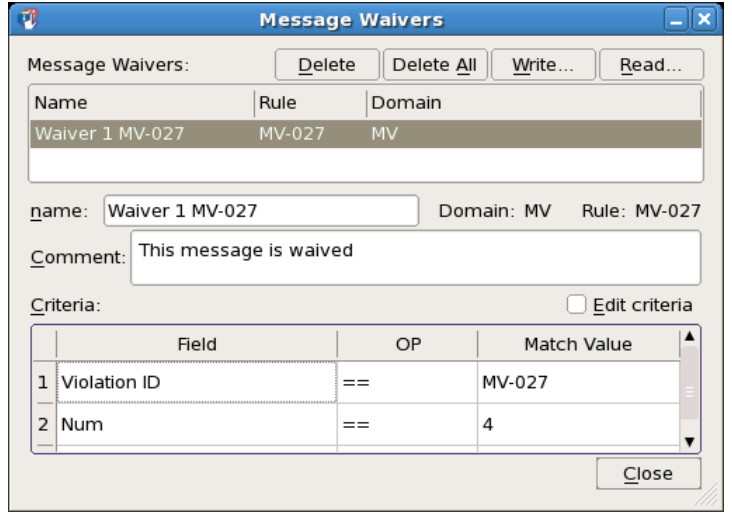
\includegraphics[width=0.92\textwidth]{gui-fig-141.png}
\caption{消息豁免列表}
\label{fig:gui-141}
\end{figure}

单击某一条豁免，可以查看创建该豁免时使用的条件。要编辑该豁免，选择 Edit criteria，修改条件设置，然后单击 Commit。也可以用这个对话框把当前豁免写成 Tcl 文件、读入保存在 Tcl 文件中的豁免，或删除当前豁免。

要在另一个会话中使用这些豁免，必须先把它们保存到磁盘。要把豁免保存到磁盘，在 Message Waivers 对话框中单击 Write，或从消息浏览器菜单选择 \textbf{File > Write Waiver to Script}。工具把 \cmd{gui\_create\_message\_waiver} 命令写入该文件。要读入保存在 Tcl 文件中的豁免，在 Message Waivers 对话框中单击 Read，或从消息浏览器菜单选择 \textbf{File > Read Waiver from Script}，然后选择包含这些豁免的 Tcl 文件。

\section{合并 EMS 数据库}
\subsection*{Merging EMS Databases}

消息浏览器可以在同一次会话中加载多个 EMS 数据库。同一时间只能有一个数据库处于活动状态。要加载不止一个数据库：
\begin{enumerate}
  \item 从菜单选择 \textbf{File > Open Message Database}。\\
        也可以用 \cmd{open\_ems\_database} 这条 Tcl 命令打开数据库，如下例所示：
\begin{lstlisting}
icc2_shell> open_ems_database MV.ems
\end{lstlisting}
  \item （可选）若已经打开多个 EMS 数据库，单击要合并的那个数据库以选中它，并从菜单选择 \textbf{File > Set Current Message Database}。
  \item 从菜单选择 \textbf{File > Merge Message Database}，选择一个文件，然后单击 OK。
\end{enumerate}

工具加载所选的数据库文件，并把它设为当前数据库，见图~\ref{fig:gui-142}。新加载的数据库文件既包含它自己原有的消息，也包含合并之前当前数据库中的消息。

\begin{figure}[htbp]
\centering
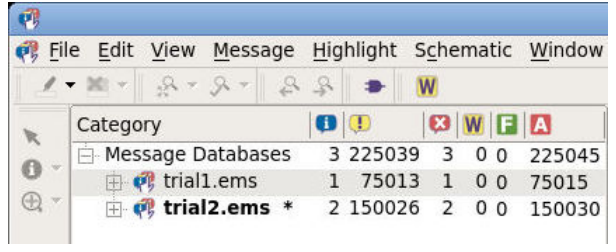
\includegraphics[width=0.92\textwidth]{gui-fig-142.png}
\caption{合并数据库}
\label{fig:gui-142}
\end{figure}

\begin{seeAlsoBox}
用 Tcl 命令管理 EMS 数据库的更多信息，见下列命令的手册页：
\begin{itemize}
  \item \cmd{close\_ems\_databases}
  \item \cmd{create\_ems\_database}
  \item \cmd{get\_current\_ems\_database}
  \item \cmd{get\_ems\_databases}
  \item \cmd{open\_ems\_database}
  \item \cmd{save\_ems\_database}
  \item \cmd{set\_current\_ems\_database}
\end{itemize}
\end{seeAlsoBox}
